%\documentclass{article}
%\usepackage{tikz,pgfplots}
%\usepackage[pdftex,active,tightpage]{preview}
%\begin{document}
%\begin{preview}

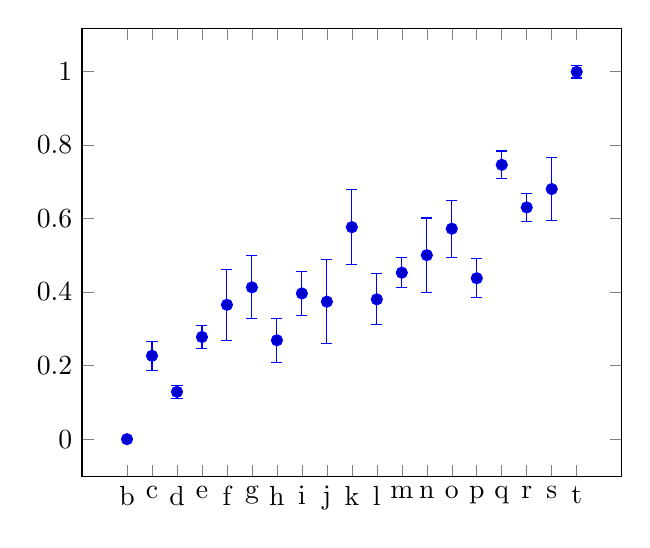
\begin{tikzpicture}
\begin{axis}[%
	%grid=both,%
	%xmajorgrids,%
	xtick={1,2,3,4,5,6,7,8,9,10,11,12,13,14,15,16,17,18,19},%
	xticklabels={b,c,d,e,f,g,h,i,j,k,l,m,n,o,p,q,r,s,t},%
]
% Line plot
\addplot
	plot[ 	%smooth,
	   		only marks,
	      	error bars/.cd,
	      	y dir=both, y explicit %
		]
	coordinates{
	(1,0) 			+- (0,0)
	(2,0.226697)	+- (0,0.0389)
	(3,0.128649)	+- (0,0.0174)
	(4,0.277819)	+- (0,0.0316)
	(5,0.365309) 	+- (0,0.0960)
	(6,0.412726)	+- (0,0.0856)
	(7,0.268849) 	+- (0,0.0598)
	(8,0.396237)	+- (0,0.0589)
	(9,0.373823)	+- (0,0.1148)
	(10,0.576375)	+- (0,0.1020)
	(11,0.380172) 	+- (0,0.0696)
	(12,0.452672)	+- (0,0.0404)
	(13,0.500303)	+- (0,0.1010)
	(14,0.572158)	+- (0,0.0778)
	(15,0.437586)	+- (0,0.0524)
	(16,0.745885)	+- (0,0.0376)
	(17,0.630023)	+- (0,0.0386)
	(18,0.679989)	+- (0,0.0852)
	(19,0.998734)	+- (0,0.0169)
};

\end{axis}
\end{tikzpicture}


% plot erstellt mit MATLAB-File p:\doc\MATLAB\WFS-CompareDMPs\wfs_Compare2008c.m (FromToTo = 1:5:1024)
% und matlab2tikz

%[ 1:19;std(NormCumulativeError);mean(NormCumulativeError)]
%
%ans =
%
%  Columns 1 through 12
%
%    1.0000    2.0000    3.0000    4.0000    5.0000    6.0000    7.0000    8.0000    9.0000   10.0000   11.0000   12.0000
%         0    0.0389    0.0174    0.0316    0.0960    0.0856    0.0598    0.0589    0.1148    0.1020    0.0696    0.0404
%         0    0.2267    0.1286    0.2778    0.3653    0.4127    0.2688    0.3962    0.3738    0.5764    0.3802    0.4527
%
%  Columns 13 through 19
%
%   13.0000   14.0000   15.0000   16.0000   17.0000   18.0000   19.0000
%    0.1010    0.0778    0.0524    0.0376    0.0386    0.0852    0.0169
%    0.5003    0.5722    0.4376    0.7459    0.6300    0.6800    0.9987          	
         	
%
%\end{preview}
%\end{document}